\section{Data generation for the sphere}
A significant challenge in this project has been obtaining high-quality data for training data-driven methods on a sphere.
To tackle this, we are exploring various approaches for data generation, including the potential to create our own data and utilize external data sources.


\subsection*{Projecting 2D data to the sphere}
Our initial approach involved projecting the solution data from the 2D SWE onto the sphere.
To ensure stability and generate high-quality data, we set the CFL number to 0.8.
The coordinates $\theta$ (longitude) and $\phi$ (latitude) are treated similarly to $x$ and $y$ in the 2D case.
The grid is configured with $N_{\theta} = 200$ grid points in the $\theta-$direction and $N_{\phi} = 100$ grid points in the $\phi-$direction.
The higher resolution in the $\theta-$direction accounts for its double distance compared to the $\phi-$direction.
We use a Gaussian function as initial condition
\begin{align*}
    h(\theta, \phi, 0) = h_0 + a \cdot \exp\left( -\frac{{(\theta - \theta_c)}^2 + {(\phi - \phi_c)}^2}{{(2\sigma)}^2} \right),
\end{align*}
where $h_0 = 1$ m, $a = 3$, $\theta_c = \frac{3 \pi}{2}, \phi_c = \frac{\pi}{3}$, and $\sigma = \frac{\pi}{16}$.
The SWE are solved from $t = 0$ s to $t_{\text{end}} = 0.5$ s, using a variable step size $\Delta t$.
The simulation takes 199 time steps, resulting in an average time step size of $\Delta t \approx 0.0025$ s.
This value is significantly smaller than in the 2D case, likely due to the higher number of grid points, another domain and lower CFL number.
The results after some given time steps are presented in~\autoref{fig:sphere_projected_water_height_timesteps}.
\begin{figure}[H]
    \centering
    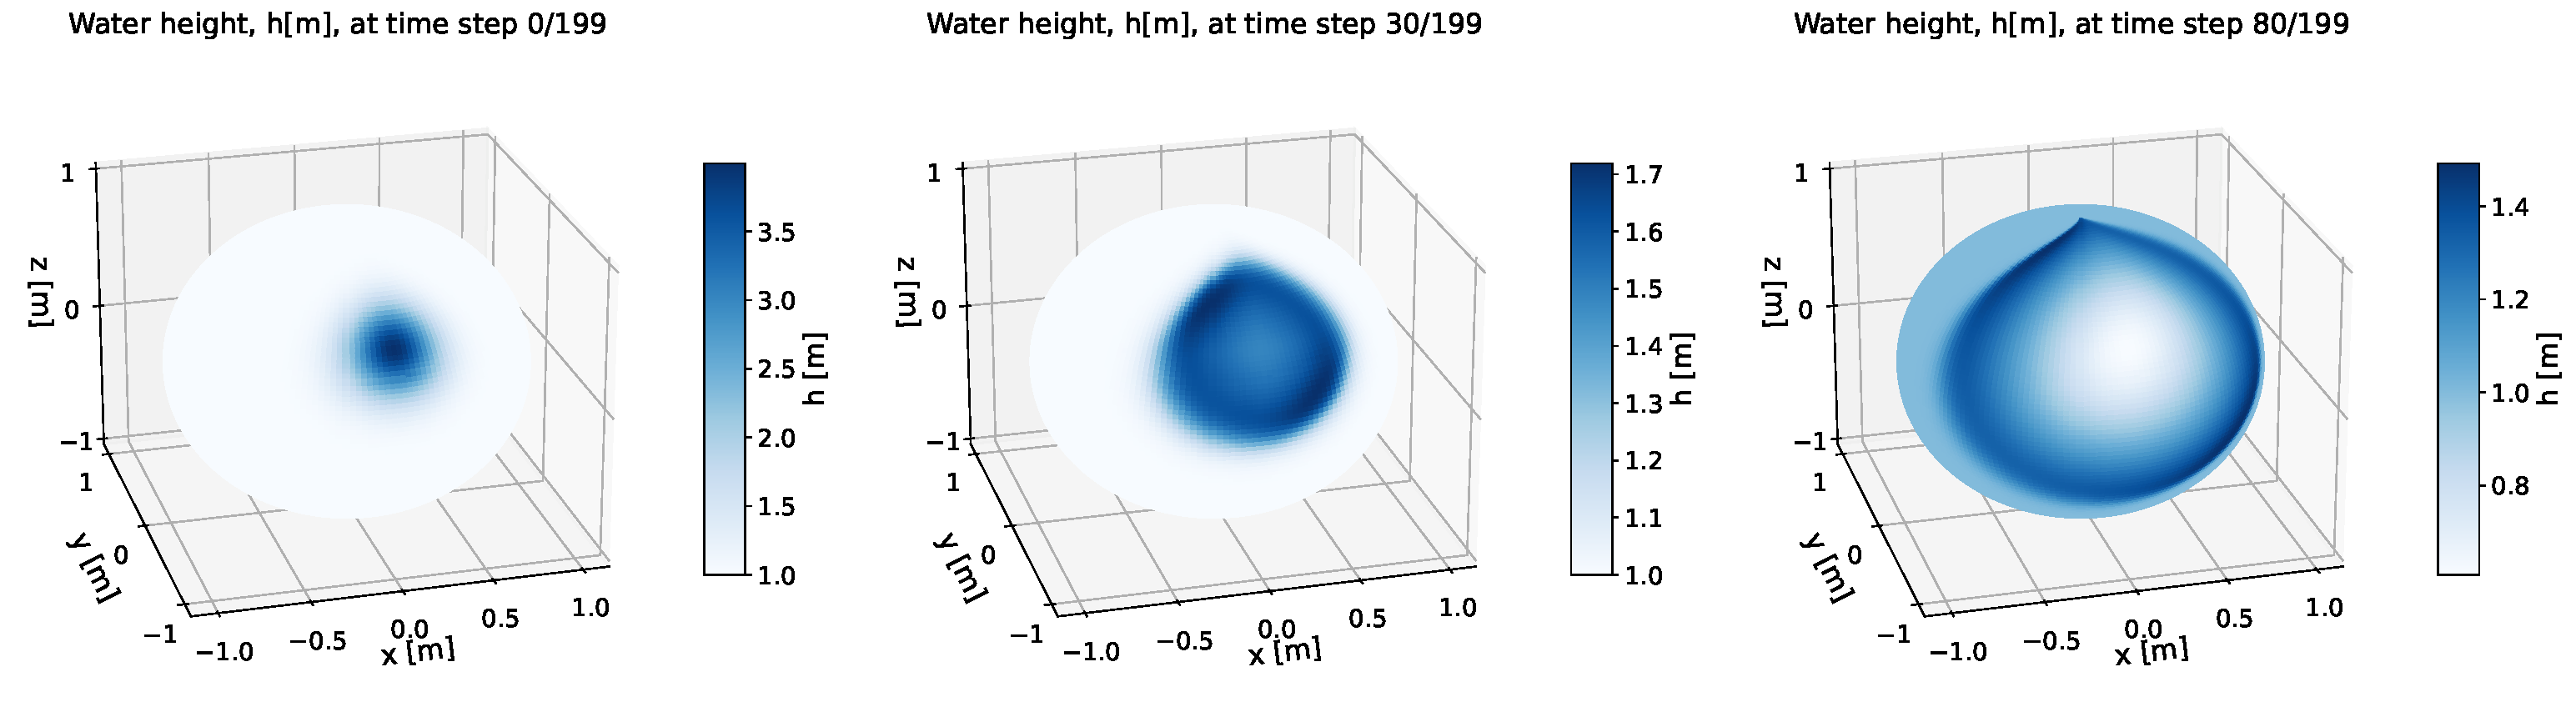
\includegraphics[width=0.95\textwidth]{C:/Users/Matteo/Shallow-Water-Equations/plots/sphere_projected_water_height_timesteps.pdf}
    \caption{Water height on the sphere for different timesteps.}\label{fig:sphere_projected_water_height_timesteps}
\end{figure}
In~\autoref{fig:sphere_projected_water_height_timesteps}we observe the evolution of the water height over time on the sphere.
The initial Gaussian bump propagates across the sphere, but singularities are present, especially at the poles.
These issues arise, amont other things, from neglecting the curvature of the sphere. 
While this approach might be acceptable for some applications, for instance when focusing on a small region near the equator, where the projection is more accurate, it is not suitable for our project.
Since our aim is to model the entire sphere, accounting for its curvature is essential.
Consequently, we cannot use this data.

\subsection*{Mesh generation for the sphere}
To solve the SWE on the sphere, we must use a different grid than the regular grid used in the 2D case.
One approach is to use an icosahedral grid, which approximates the sphere with triangles.
The grid structure allows for various levels of refinement, depending on the desired level of accuracy.
At each refinement level, the number of triangles increases by a factor of four, as each triangle is divided into four smaller triangles, meaning that the number of triangles increases drastically with each level of refinement.
The grid is generated using Matlab code from the Github repository~\cite{sphere_mesh_triangles} and then rewritten to Python.
The first four levels of refinement are shown in~\autoref{fig:icosahedral_grid}.
\begin{figure}[H]
    \centering
    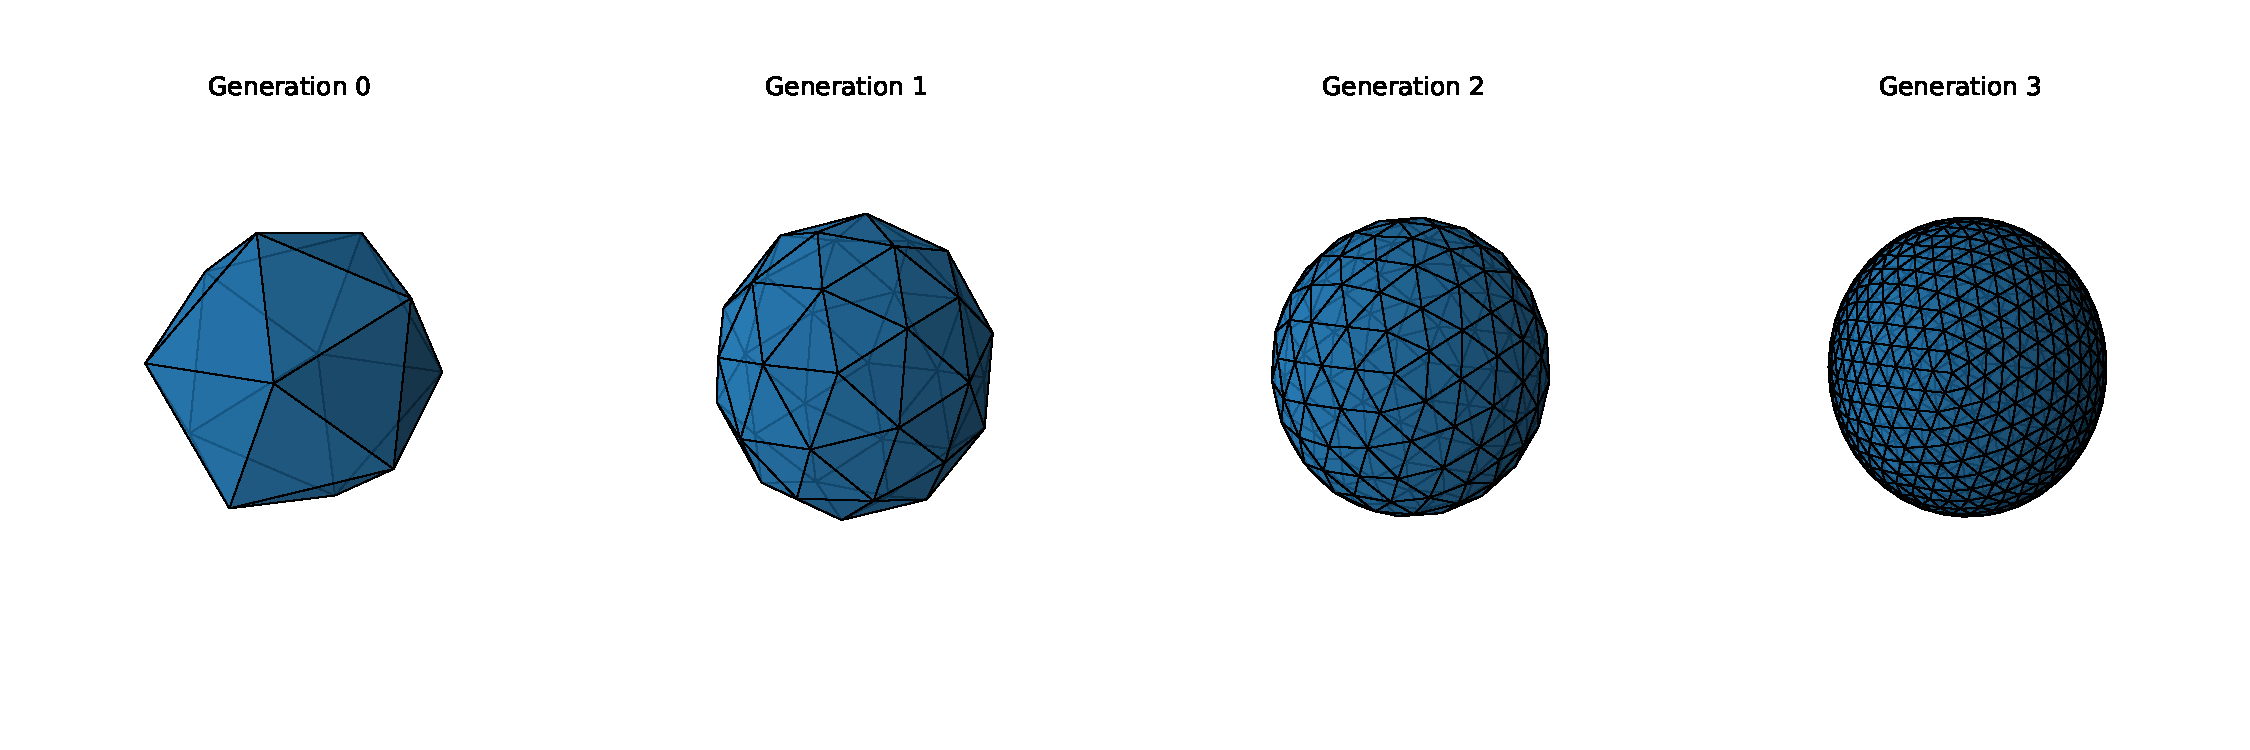
\includegraphics[width=\textwidth]{C:/Users/Matteo/Shallow-Water-Equations/plots/icosahedral_mesh_refinement.pdf}
    \caption{Icosahedral grid for the first 4 levels of refinement.}\label{fig:icosahedral_grid}
\end{figure}
In~\autoref{fig:icosahedral_grid} we see how the grid is refined at each level, resulting in a progressively more accurate representation of the sphere.
We will brieftly outline the process of solving the SWE on this grid structure, inspired by the finite element method (FEM).


We will shortly outline the process of solving the SWE on this grid structure, inspired by the finite element method (FEM).
The main idea is that for each triangle we keep track of which the neighboring triangles are. 
We also keep track of which interfaces the neighboring triangles share. 
This information is stored in various tables, known as the Element-to-Vertex, Element-to-Face, and Element-to-Element tables.
Each triangle is numbered, as well as each vertex.
The Element-to-Vertex (EToV) table stores the vertices of each triangle, meaning that each row corresponds to a triangle and the three columns correspond to the three vertices of the triangle.
The Element-to-Element (EToE) table can be made based on the EToV table.
The EToE table stores the neighboring triangles of each triangle, meaning that each row corresponds to a triangle and the three columns correspond to the three neighboring triangles, using the given labeling.
The Element-to-Face (EToF) table keeps track of which faces (edges) that are shared between two triangles, meaning for each triangle for each neighbor we must know which face the two triangles share.

The idea is then that for each interface we compute the fluxes between the triangles.
That is, we calcualte the fluxes the goes out of one triangle and into the neighbor.
This is to make sure the total flux overall is zero, meaning that the total volume of water is conserved.
However, we must be aware of the fact that the triangles are not on straigt lines, like the case in 2D. 
Meaning for each flux on each interface we must compute the contribution in the $\theta-$ and the $\phi-$direction.
Where previous we could more or less view the overall problem as two 1D problems, now they are interchanged.




\subsection*{External data sources}


\begin{figure}[H]
    \centering
    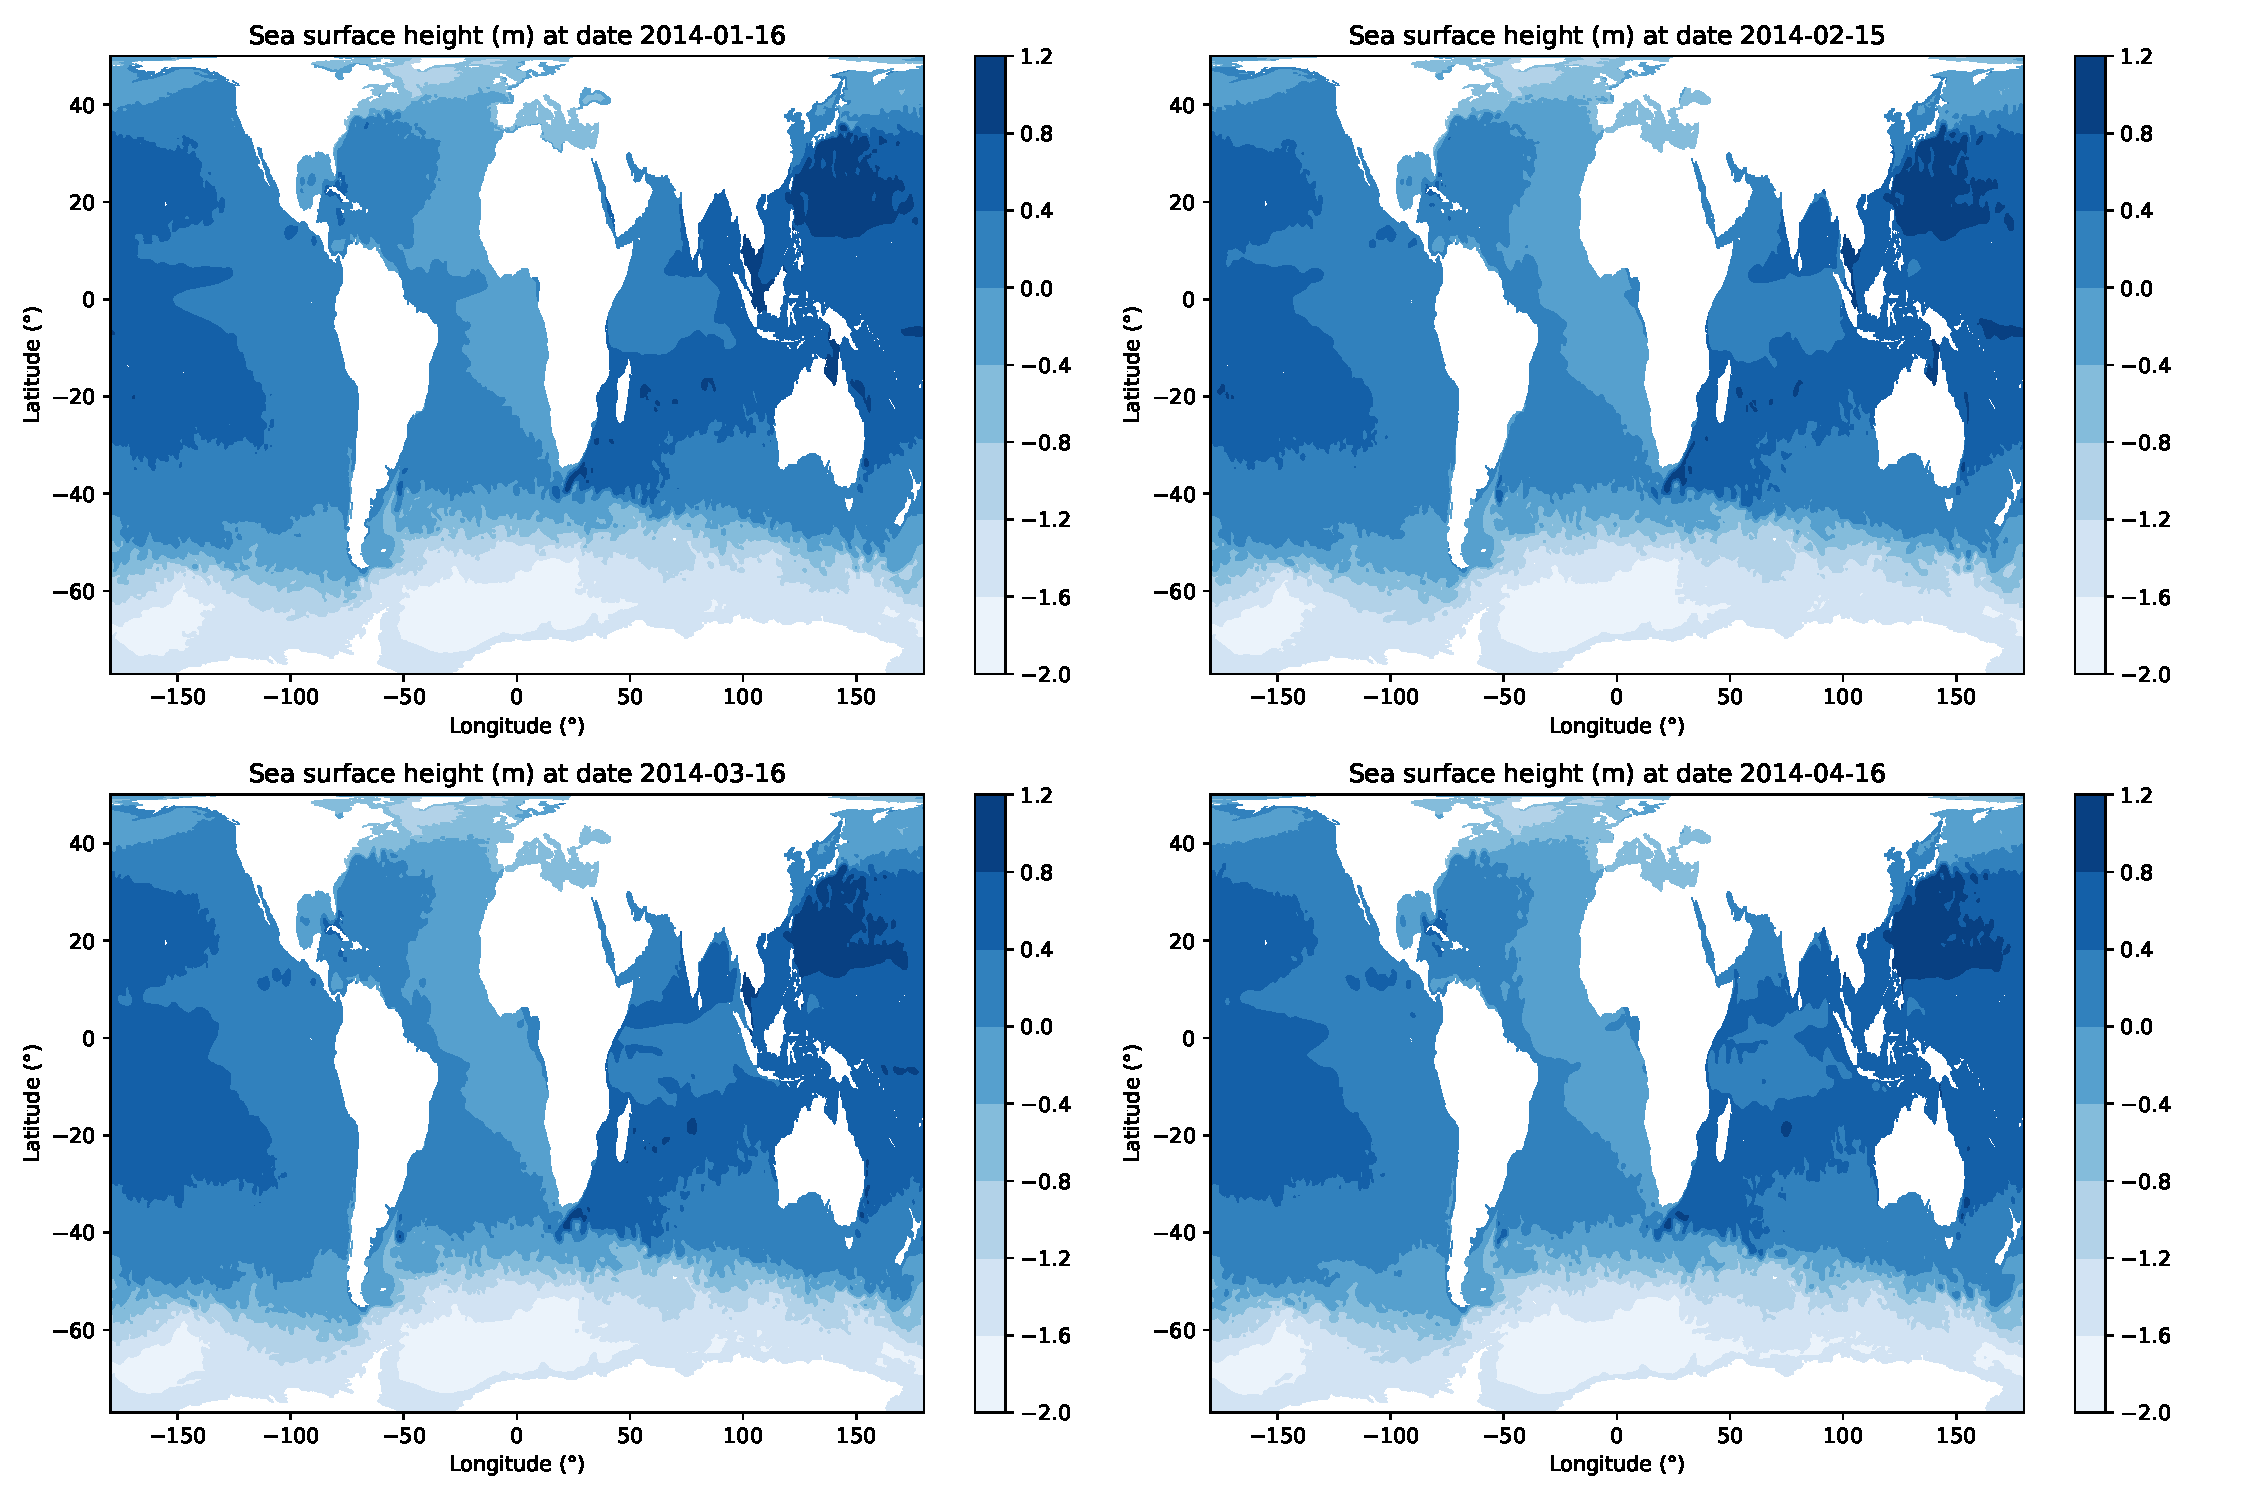
\includegraphics[width=0.95\textwidth]{C:/Users/Matteo/Shallow-Water-Equations/plots/ssh_field.pdf}
    \caption{Sea surface height as the diffference from reference sea surface height for the months Jan-Apr 2014.}\label{fig:copernices-ssh}
\end{figure}


